\documentclass[12pt,letterpaper]{article}
\usepackage[latin1]{inputenc}
\usepackage{amsmath}
\usepackage{amsfonts}
\usepackage{amssymb}
\usepackage{makeidx}
\usepackage{graphicx}
\usepackage[normalem]{ulem}
\usepackage{setspace}
\usepackage{subcaption}
\usepackage{float}
\usepackage{titlesec}
\usepackage[margin=1in]{geometry}
\usepackage{hyperref}
\usepackage{ntheorem}
\newtheorem{hyp}{Hypothesis}
\newtheorem{subhyp}{Hypothesis}[hyp]
\renewcommand\thesubhyp{\thehyp.\alph{subhyp}}
\usepackage[round]{natbib}
\bibpunct{(}{)}{;}{a}{}{,~}
\usepackage[space]{grffile}
\graphicspath{{./figures/}}
\usepackage[affil-it]{authblk}
\makeatletter
\def\@maketitle{%
	\newpage
	\null
	\vskip 2em%
	\begin{center}%
		\let \footnote \thanks
		{\Large\bfseries \@title \par}%
		\vskip 1.5em%
		{\normalsize
			\lineskip .5em%
			\begin{tabular}[t]{c}%
				\@author
			\end{tabular}\par}%
		\vskip 1em%
		{\normalsize \@date}%
	\end{center}%
	\par
	\vskip 1.5em}
\makeatother

\title{Coordination in Conflict Theaters: Explaining Contributions to Coalition Warfare}

\author{J Andr\'{e}s Gannon%
	\thanks{Electronic address: \texttt{jagannon@ucsd.edu}}}
\affil{Department of Political Science \\ University of California, San Diego}

\author{Daniel Kent%
	\thanks{Electronic address: \texttt{kent.249@osu.edu} \\ Acknowledgments. This research was sponsored by Office of Naval Research Grant N00014-14-1-0071 and the Department of Defense Minerva Research Initiative. Any opinions, findings, and conclusions or recommendations expressed in this publication are those of the authors and do not necessarily reflect the view of the Office of Naval Research.}}
\affil{Department of Political Science \\ Ohio State University}

\begin{document}
\maketitle

\begin{abstract}

\end{abstract}

\section{Introduction}
Kitchy example of country that contributed a lot of its forces despite having no stake in the fight and no formal obligation to do so. Denmark and New Zealand contributed the highest percent of their military to ISAF, over 0.6%
Greece, Poland, Belgium, Bulgaria, Portugal, and the Czech Republic contributed less than 0.1%

We think that countries participate in war because they care about the outcome or because they want to support their friends. But they also sometimes to do not to support their friends, but to make friends.

?...good opportunity for the New Zealand Defence Force to test its interoperability with contributing NATO nations. This deployment is an example of New Zealand?s commitment to playing our part in supporting NATO in areas of common interest.? -- Jonathan Coleman, New Zealand Defence Minister


Paper examines troop contributions during the first half of the Afghan war to see what explains the degree of a country's contribution. Innovation is in not looking at overall troop count, which biases towards larger countries, but instead looking at degree of contribution relative to the size of that country's armed forces. Finds that countries that wanted to make new friends with central actors overcontribute a larger size of their armed forces relative to countries who had a stake in the fight and were formally obligated to fight alongside their friends.

Has implications for how we think about alliances and coalition warfare. We think of war as a costly tool for achieving international objectives. One of these objectives is signaling to warfighters that you are willing to undergo a large cost to help them achieve their goal with the hopes that it improves your relationship with them in the future. War can be a good excuse for making new friends

Paper proceeds in a few parts, etc.

\section{Existing Studies on Coalition Warfare}
Why do countries fight together in coalitions

Those that want to win

Formal obligation from alliance conditions

Assumes countries that fight together are already predisposed to have aligned interests. Doesn't look at how fighting together can alter the alignment of interests.

Some work has looked at related areas like UN peacekeeping, we apply it in a different context where its easier to separate formal obligation from wanting to signal closer friendships, its easier to identify the central actor, and the costs are higher

\section{Theory of Signaling via Coalition Contributions}
Nature of military contribution to conflict theater is predicted by a nation?s location in security community because that determines its primary international objective

Central vs peripheral
	\begin{figure}[H]
		\centering
		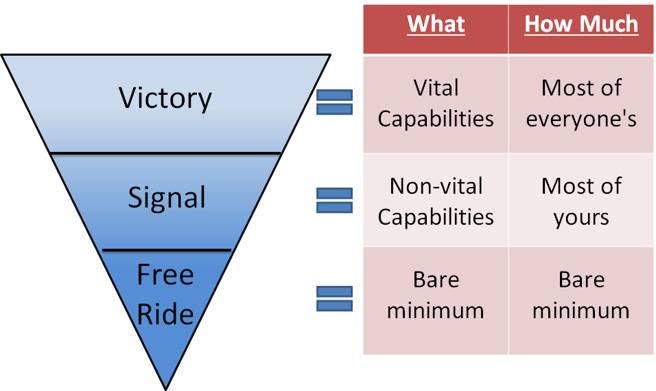
\includegraphics[width=0.6\textwidth]{contribution_pyramid.png}
		\caption{Theory of Coalition Warfare Contributions}
		\label{fig:theory}
	\end{figure}			

\section{Research Design}
Unit of analysis: State (2001-2005)

DV: Percent of national military personnel fighting in Afghanistan War

EV: Preference Alignment with US/UK + Military pact with US/UK
Controls: Military Pact, Ideal Point Distance from US,  Eigenvector Centrality in Preference Network, CINC score, Distance from Afghanistan

Model: pact + ideal point + pact*ideal point + eigen + cinc + log(distance)


\section{Results}


\section{Conclusion}
Takeaway -- Small states fight for future military cooperation
Contribution -- New data on relative contributions helps explain free-riding exceptions
Future work -- Does this payoff? Look at other coalition wars

?In the Libya operation, Norway and Denmark, have provided 12 percent of allied strike aircraft yet have struck about one third of the targets...These countries have, with their constrained resources, found ways to do the training, buy the equipment, and field the platforms necessary to make a credible military contribution.? -- US Defence Secretary Robert Gates (June 2011)


\bibliographystyle{apsr}
\bibliography{mctl_alliances_bib}

\end{document}
